\chapter{Anhang}\label{ch:appendix}
\section{Übertragung der Nachrichten}\label{sec:msg-trans}

\vspace{1cm}
\begin{samepage}
	\thispagestyle{empty}
	\begin{figure}[htbp]
		\centering
		\scalebox{\scalepic}{
			\begin{tikzpicture}
				\tikzset{func/.style={rectangle, draw, fill=func-red, rounded corners}}
				\tikzset{arr/.style={-{Stealth[scale=1]}, thick, shorten <=.1cm, shorten >=.1cm}}
				\tikzset{think/.style={cloud callout, callout relative pointer={(0.2, -0.8)}, cloud puff arc=120, aspect=1.5, align=center, fill=white, draw}}
				
				\node at +(0,.5cm) (alice){};
				\node[think, above=1.8cm of alice] {$K_S$};
				\Strichmaxerl[5] 
				\node[below] at (-0.3, 0) {Alice};
				\node[func, right=of alice] at +(0, .5cm) (enigma) {Enigma};
				\draw[arr] (alice) -- node[above] {$K_S$} (enigma);
				\draw[arr] (enigma.north)+(0, .7cm) node[above] {$K_T$} -- (enigma);
				\node[right=2cm of enigma] (dest) {};
				\draw[arr] (enigma.east) -- node[above] {$K_T + K_S^\prime$} (dest);
				\draw[gray] 
				(dest)++(0,-0.2cm)
				-- ++(0,0.5cm) 
				-- ++(2cm,0) 
				-- ++(0,-0.5cm) 
				-- ++(-0.5cm, 0.1cm) 
				-- ++(-0.5cm, -0.1cm) 
				node[above=.1cm, black] {\tiny Spruchkopf}
				-- ++(-0.5cm, 0.2cm) 
				-- ++(-0.5cm, -0.2cm)
				-- cycle;
			\end{tikzpicture}
		}
		\caption{Erzeugung Spruchkopf}
		\label{fig:msg-head}
	\end{figure}
	\begin{figure}[htbp]
		\centering
		\scalebox{\scalepic}{
			\begin{tikzpicture}
				\tikzset{func/.style={rectangle, draw, fill=func-red, rounded corners}}
				\tikzset{arr/.style={-{Stealth[scale=1]}, thick, shorten <=.1cm, shorten >=.1cm}}
				\node at +(0,.5cm) (alice){};
				\Strichmaxerl[5] 
				\node[below] at (-0.3, 0) {Alice};
				\node[func, right=of alice] (enigma) {Enigma};
				\draw[arr] (alice) -- node[above] {$M$} (enigma);
				\draw[arr] (enigma.north)+(0, .7cm) node[above] {$K_S$} -- (enigma);
				\node[right=of enigma] (dest) {};
				\draw[arr] (enigma.east) -- node[above] {$M^\prime$}(dest);
				\draw[gray] 
				(dest)++(0,0.2cm) 
				-- ++(0,-1cm) 
				-- ++(2cm,0)
				-- ++(0,1cm)
				-- ++(-0.5cm, 0.1cm) 
				-- ++(-0.5cm, -0.1cm) 
				-- ++(-0.5cm, 0.2cm) 
				-- ++(-0.5cm, -0.2cm)
				-- cycle; 
			\end{tikzpicture}
		}
		\caption{Chiffrierung Nachricht}
		\label{fig:enc-msg}
	\end{figure}
	\begin{figure}[htbp]
		\centering
		\scalebox{\scalepic}{
			\begin{tikzpicture}
				\tikzset{func/.style={rectangle, draw, fill=func-red, rounded corners}}
				\tikzset{arr/.style={-{Stealth[scale=1]}, thick, shorten <=.1cm, shorten >=.1cm}}
				
				\node at +(-0.3,.5cm) (bob){};
				\Strichmaxerl[5] 
				\node[below] at (-0.3, 0) {Bob};
				\node[func, left=of bob] (enigma) {Enigma};
				\draw[arr] (enigma) -- node[above] {$K_S$}(bob);
				\draw[arr] (enigma.north)+(0, .7cm) node (top env) {} -- node[right, midway] {$K_T$} (enigma);
				\draw[gray] 
				(top env)++(-1cm,0)
				-- ++(0,0.5cm) 
				-- ++(2cm,0) 
				-- ++(0,-0.5cm) 
				-- ++(-0.5cm, 0.1cm) 
				-- ++(-0.5cm, -0.1cm) 
				node[above=.1cm, black] {\tiny Spruchkopf}
				-- ++(-0.5cm, 0.2cm) 
				-- ++(-0.5cm, -0.2cm)
				-- cycle;
				\coordinate (top env start) at (enigma.north)+(-1cm, .7cm);
				\node[] at (top env start) (top env) {};
				
				\node[left=of enigma] (dest) {};
				\draw[arr] (dest) -- node[above] {$K_S^\prime$} (enigma);
				\node[left=1.7cm of dest] (bottom env) {};
				\draw[gray] 
				(bottom env)++(0,-0.2cm) 
				-- ++(0,0.5cm) 
				-- ++(2cm,0) 
				-- ++(0,-0.5cm) 
				-- ++(-0.5cm, 0.1cm) 
				-- ++(-0.5cm, -0.1cm) 
				node[above=.1cm, black] {\tiny Spruchkopf}
				-- ++(-0.5cm, 0.2cm) 
				-- ++(-0.5cm, -0.2cm)
				-- cycle;
			\end{tikzpicture}
		}
		\caption{Dechiffrierung Spruchschlüssel}
		\label{fig:dec-head}
	\end{figure}
	\begin{figure}[H]
		\centering
		\scalebox{\scalepic}{
			\begin{tikzpicture}
				\tikzset{func/.style={rectangle, draw, fill=func-red, rounded corners}}
				\tikzset{arr/.style={-{Stealth[scale=1]}, thick, shorten <=.1cm, shorten >=.1cm}}
				\node at +(-0.3,.5cm) (bob){};
				\Strichmaxerl[5] 
				\node[below] at (-0.3, 0) {Bob};
				\node[func, left=of bob] (enigma) {Enigma};
				\draw[arr] (enigma.north)+(0, 1cm) -- node[right, midway] {$K_S$} (enigma);
				\draw[arr] (enigma) --  node[above] {$M$} (bob);
				\node[left=of enigma] (dest) {};
				\draw[arr] (dest) -- node[above] {$M^\prime$} (enigma);
				\node[left=1.7cm of dest] (bottom env) {};
				\draw[gray] 
				(bottom env)++(0,0.2cm) 
				-- ++(0,-1cm) 
				-- ++(2cm,0)
				-- ++(0,1cm)
				-- ++(-0.5cm, 0.1cm) 
				-- ++(-0.5cm, -0.1cm) 
				-- ++(-0.5cm, 0.2cm) 
				-- ++(-0.5cm, -0.2cm)
				-- cycle; 
			\end{tikzpicture}
		}
		\caption{Dechiffrierung Nachricht}
		\label{fig:dec-msg}
	\end{figure}
\end{samepage}

\section{Laufzeit Menü Algorithmus}\label{sec:runtime_menu}
\begin{figure}[htbp]
	\centering
	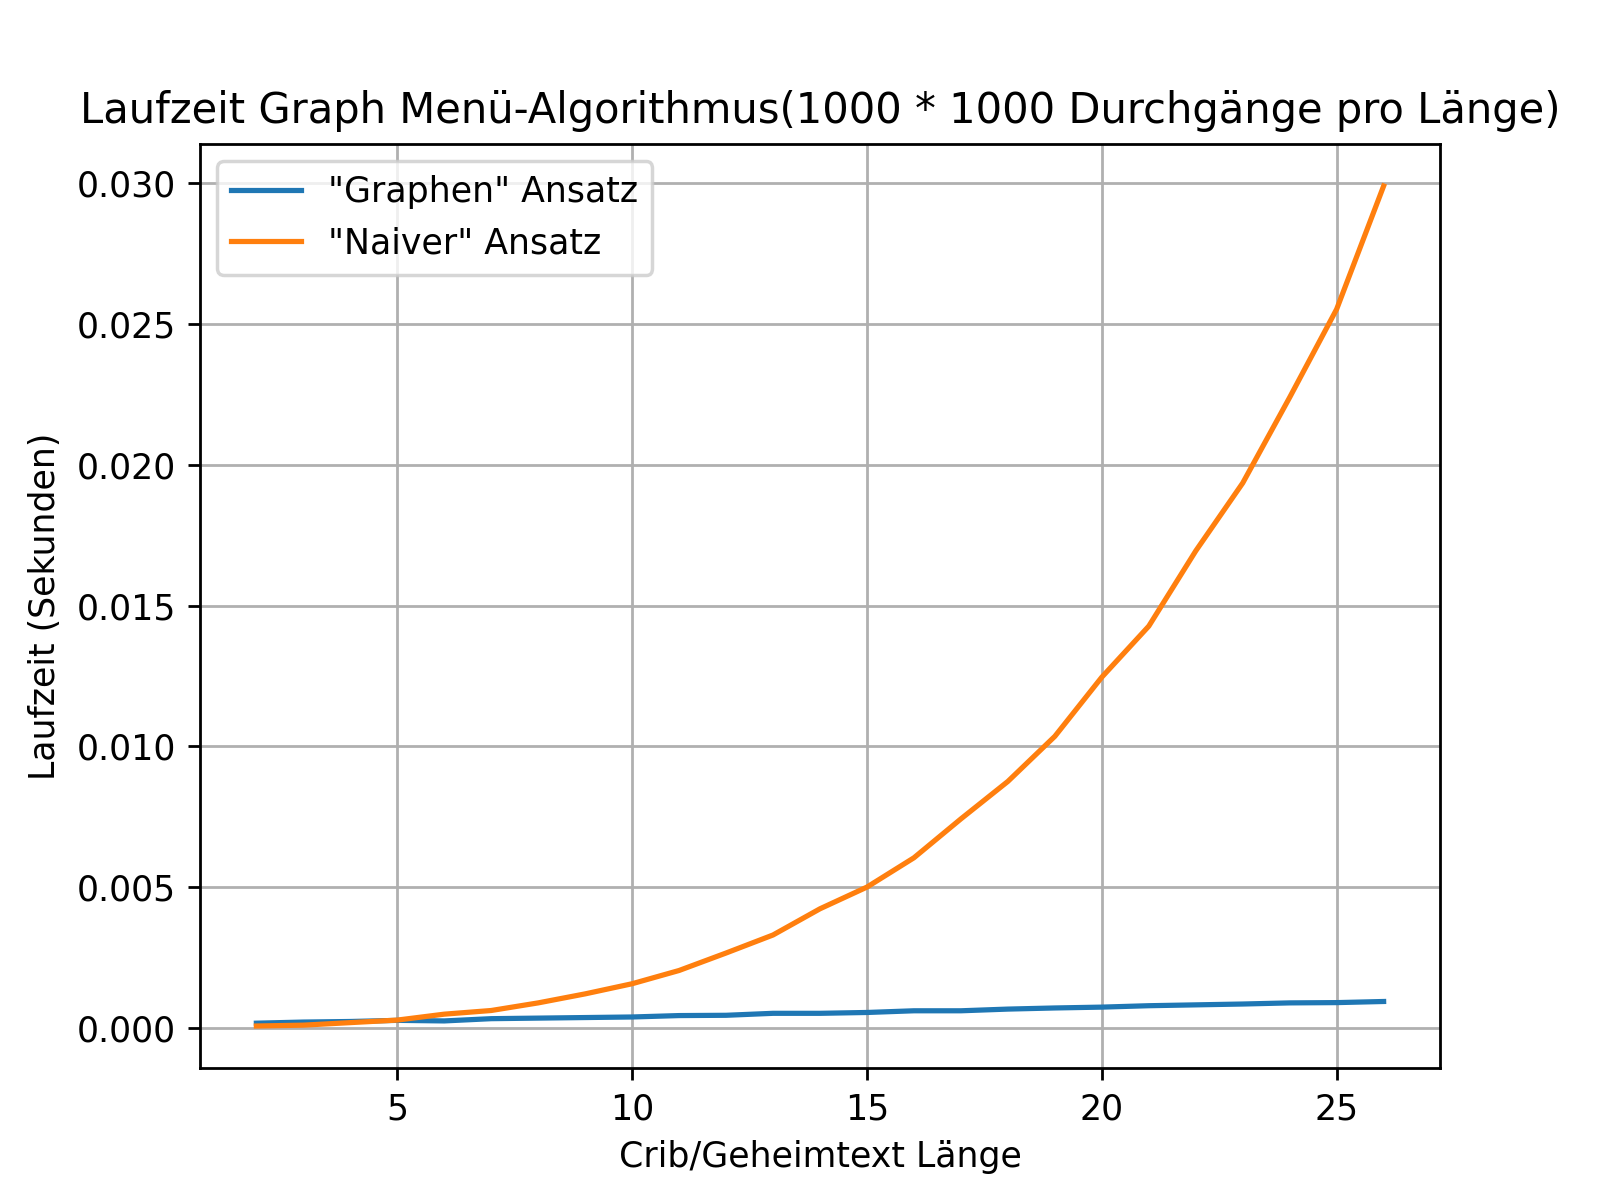
\includegraphics[width=.7\linewidth]{Turing Bomb/Crib-Cipher Loop/Runtime Graph Graph vs Force}
	\caption{Laufzeit-Graph Menü-Algorithmus}
	\label{fig:app_menu_runtime}
\end{figure}
Es wurden pro Länge 1000 Zufalls Crib und Geheimtexte generiert und diese
jeweils mit 1000 Durchgängen getestet.